\documentclass[10pt,a4paper]{article}
\usepackage[margin=18mm,headheight=14pt,footskip=12mm]{geometry}
\usepackage[T1]{fontenc}
\usepackage{lmodern}
\renewcommand{\familydefault}{\sfdefault}
\usepackage{microtype}
\usepackage{tikz}
\usetikzlibrary{arrows.meta,positioning,calc,fit}
\usepackage{tabularx,longtable,array,booktabs}
\usepackage[most]{tcolorbox}
\usepackage{enumitem}
\usepackage{hyperref}
\usepackage{fancyhdr}
\usepackage{needspace}
\usepackage{xcolor}
\usepackage{graphicx}
\definecolor{ink}{HTML}{142426}
\definecolor{teal}{HTML}{087C76}
\definecolor{mint}{HTML}{E8F5F1}
\definecolor{lime}{HTML}{D6ED81}
\definecolor{coral}{HTML}{D46B56}
\definecolor{pale}{HTML}{F5F7F4}
\definecolor{line}{HTML}{CDDAD5}
\definecolor{muted}{HTML}{536467}
\hypersetup{colorlinks=true,linkcolor=teal,urlcolor=teal,pdftitle={Webby Voicer Figma and Rive Handoff},pdfauthor={Webby Voicer project}}
\pagestyle{fancy}
\fancyhf{}
\fancyhead[L]{\small\color{muted} WEBBY VOICER / DESIGN HANDOFF}
\fancyhead[R]{\small\color{muted} DUB MODE BETA}
\fancyfoot[L]{\small\color{muted} 03 OCT 2026}
\fancyfoot[R]{\small\color{muted}\thepage}
\renewcommand{\headrulewidth}{0.4pt}
\setlength{\parindent}{0pt}
\setlength{\parskip}{5pt}
\setlist[itemize]{leftmargin=16pt,itemsep=2pt,topsep=3pt}
\setlist[enumerate]{leftmargin=17pt,itemsep=2pt,topsep=3pt}
\newcommand{\kicker}[1]{\vspace{5pt}{\small\bfseries\color{teal}#1}\par\vspace{2pt}}
\newcommand{\screen}[2]{\Needspace{60pt}\subsection*{\color{ink}#1\quad #2}}
\newtcolorbox{callout}[1][]{colback=mint,colframe=line,boxrule=0.7pt,arc=3pt,left=8pt,right=8pt,top=6pt,bottom=6pt,#1}
\newtcolorbox{riskbox}[1][]{colback=coral!8,colframe=coral!45,boxrule=0.7pt,arc=3pt,left=8pt,right=8pt,top=6pt,bottom=6pt,#1}
\newcommand{\contract}[3]{\begin{tabularx}{\linewidth}{@{}>{\bfseries\color{teal}}p{27mm}X@{}}Content & #1\\[3pt]Actions & #2\\[3pt]States & #3\end{tabularx}}
\tikzset{
  flow/.style={draw=line,fill=pale,rounded corners=4pt,thick,text=ink,align=center,text width=23mm,minimum height=11mm,inner sep=4pt},
  special/.style={flow,fill=mint,draw=teal},
  phase/.style={draw=line,fill=pale,rounded corners=4pt,thick,text=ink,align=center,text width=31mm,minimum height=12mm,inner sep=5pt},
  edge/.style={-{Stealth[length=2.4mm]},thick,draw=teal},
  note/.style={font=\scriptsize,text=muted,align=center}
}

\begin{document}
\pagenumbering{roman}
\begin{titlepage}
\vspace*{24mm}
{\Large\bfseries\color{teal} WEBBY VOICER\par}
\vspace{8mm}
{\fontsize{34}{38}\selectfont\bfseries\color{ink} Figma + Rive\\design handoff\par}
\vspace{7mm}
{\Large\color{muted} Dub Mode public beta / desktop + phone\par}
\vspace{17mm}

\begin{tikzpicture}
\fill[teal] (0,0) rectangle (16.5,0.18);
\fill[lime] (0,0) rectangle (5.3,0.18);
\end{tikzpicture}
\vspace{12mm}
\begin{callout}
\textbf{Purpose.} Design every user-facing beta flow and its states in Figma. Supply optional Rive motion assets with a documented app-facing contract. The current web UI is a functional placeholder; its styling and layout do not constrain the design.
\end{callout}
\vspace{7mm}
\begin{tabularx}{\linewidth}{@{}>{\bfseries}p{34mm}X@{}}
Product & Independent, free browser dubbing game; no account.\\
Release & Dub Mode, anonymous multiplayer, pack market, local import, video export.\\
Later & Classic Mode and creator submissions are outside this handoff.\\
Evidence & A supplied 1:15 Dub pack with 22 lines, two roles, icon, subtitle, line images, mixed OGG/MP3 audio, backing track, and OGV video imports and plays locally.\\
\end{tabularx}
\vfill
{\small\color{muted}Version 1.0 / 03 October 2026\par}
\end{titlepage}

\setcounter{page}{2}
\tableofcontents
\clearpage
\pagenumbering{arabic}

\section{Design boundary and product rules}
\begin{callout}
\textbf{Design principle:} Make dubbing feel playful and social while leaving the current line, recording state, and next action unmistakable. Optimize for a first-time player on a phone and a host managing eight performers on desktop.
\end{callout}
\begin{tabularx}{\linewidth}{@{}>{\bfseries\color{teal}}p{35mm}X@{}}
Account & None. A stage name exists only in a room.\\
Pack sources & Players can import a legacy Dub ZIP or folder. Market cards always link to the original GameBanana page. No creator submissions and no category exclusion at launch. A mirror is offered only when creator or license permission exists.\\
Compatibility & A pack can contain an OGV video, voice clips, timestamps, backing audio, icon, subtitle, and per-line images. Some browsers must convert OGV locally before playback/export.\\
Room & Six-character code; up to eight performers plus spectators. Host can assign/reassign roles, lock joins, choose one-line turns or simultaneous recording, and enable reactions/voting. Voting defaults off.\\
Privacy & No live microphone broadcast. Only submitted takes are heard by others. Shared pack and takes are automatically removed when the room ends or expires.\\
Result & Dub Mode has no automatic score. Finished scene has captions and creator credit. Performers see export; spectators watch without an export control.\\
\end{tabularx}
\begin{riskbox}
\textbf{Out of scope:} sign-in, paid pack checkout, public pack submission, automatic score, live voice chat, or a built-in GameBanana file mirror without permission.
\end{riskbox}

\section{Information architecture}
Page IDs are stable design labels, not required URL paths. A page may become a route, full-screen view, or overlay if its flow remains clear.
\begin{center}
\resizebox{\linewidth}{!}{%
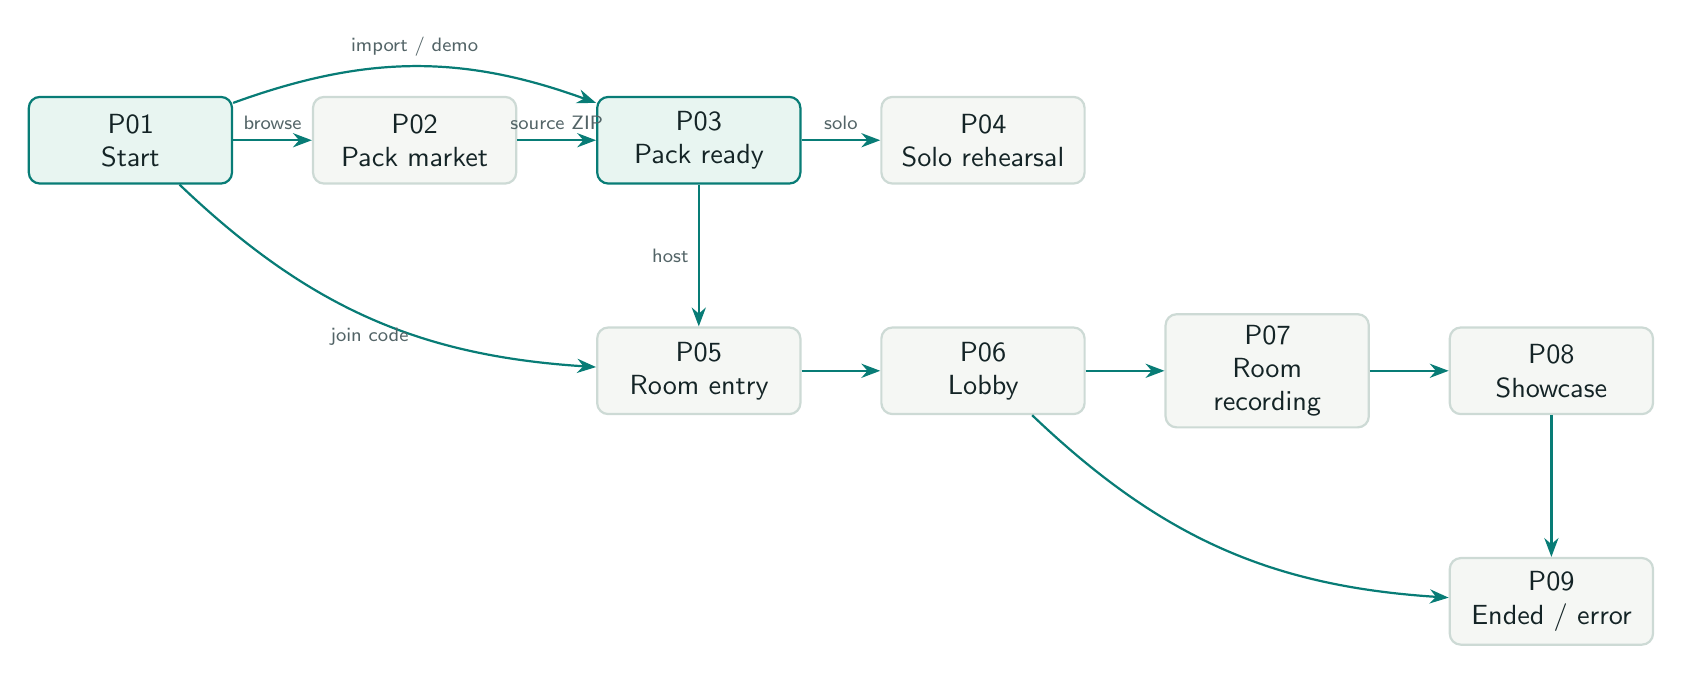
\begin{tikzpicture}[node distance=9mm and 10mm]
\node[special] (start) {P01\\Start};
\node[flow,right=of start] (market) {P02\\Pack market};
\node[special,right=of market] (ready) {P03\\Pack ready};
\node[flow,right=of ready] (solo) {P04\\Solo rehearsal};
\node[flow,below=18mm of ready] (entry) {P05\\Room entry};
\node[flow,right=of entry] (lobby) {P06\\Lobby};
\node[flow,right=of lobby] (record) {P07\\Room recording};
\node[flow,right=of record] (show) {P08\\Showcase};
\node[flow,below=18mm of show] (end) {P09\\Ended / error};
\draw[edge] (start)--node[above,note]{browse}(market);
\draw[edge] (market)--node[above,note]{source ZIP}(ready);
\draw[edge] (start) to[bend left=20] node[above,note]{import / demo} (ready);
\draw[edge] (ready)--node[above,note]{solo}(solo);
\draw[edge] (ready)--node[left,note]{host}(entry);
\draw[edge] (start) to[bend right=20] node[below,note]{join code}(entry);
\draw[edge] (entry)--(lobby);
\draw[edge] (lobby)--(record);
\draw[edge] (record)--(show);
\draw[edge] (show)--(end);
\draw[edge] (lobby) to[bend right=20] (end);
\end{tikzpicture}}
\end{center}
\kicker{Navigation requirements}
\begin{itemize}
\item From P01, import/demo, join code, and pack market are visible without opening a menu.
\item P03 presents two clear branches: rehearse alone or host with this pack.
\item A joined room keeps its code, phase, connection state, and exit path visible.
\item P09 explains media deletion and expiry; it must not suggest that a deleted room can be restored.
\end{itemize}

\section{Core interaction flows}
\subsection{Solo pack and recording}
\begin{center}
\resizebox{\linewidth}{!}{%
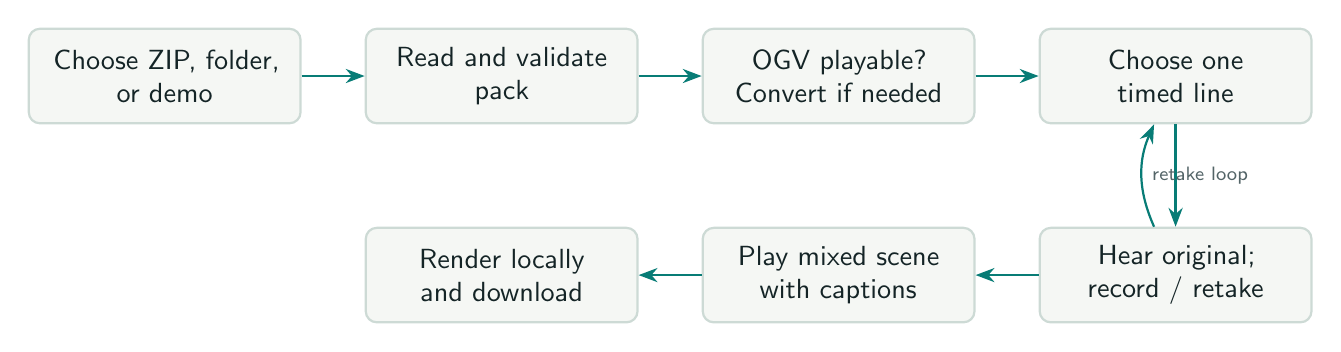
\begin{tikzpicture}[node distance=8mm]
\node[phase] (choose) {Choose ZIP, folder,\\or demo};
\node[phase,right=of choose] (parse) {Read and validate\\pack};
\node[phase,right=of parse] (convert) {OGV playable?\\Convert if needed};
\node[phase,right=of convert] (line) {Choose one\\timed line};
\node[phase,below=13mm of line] (take) {Hear original;\\record / retake};
\node[phase,left=of take] (mix) {Play mixed scene\\with captions};
\node[phase,left=of mix] (export) {Render locally\\and download};
\draw[edge] (choose)--(parse);
\draw[edge] (parse)--(convert);
\draw[edge] (convert)--(line);
\draw[edge] (line)--(take);
\draw[edge] (take)--(mix);
\draw[edge] (mix)--(export);
\draw[edge] (take) to[bend left=24] node[right,note]{retake loop} (line);
\end{tikzpicture}}
\end{center}
\textbf{Timing rule:} line timestamps can overlap. The timeline is chronological, but the UI must not assume each line has a unique whole-second slot.

\subsection{Anonymous room}
\begin{center}
\resizebox{\linewidth}{!}{%
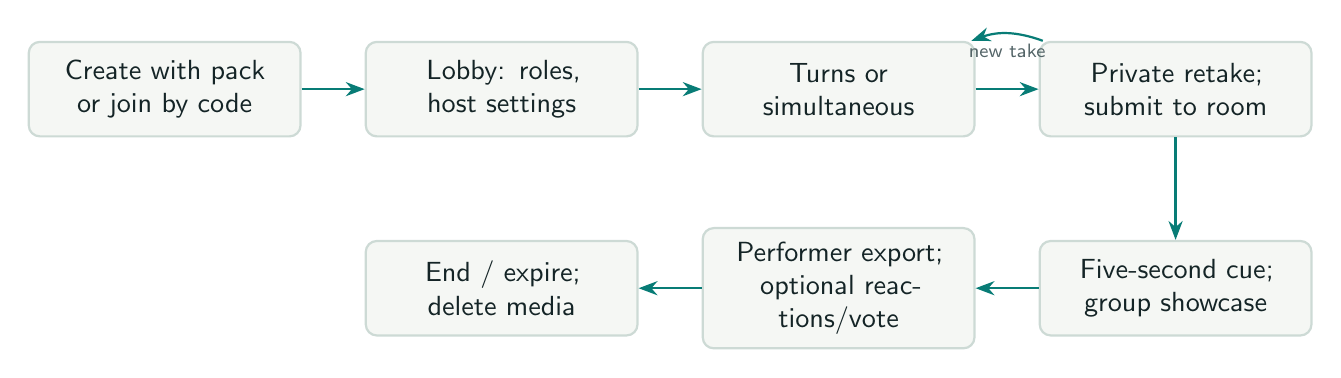
\begin{tikzpicture}[node distance=8mm]
\node[phase] (entry) {Create with pack\\or join by code};
\node[phase,right=of entry] (lobby) {Lobby: roles,\\host settings};
\node[phase,right=of lobby] (rec) {Turns or\\simultaneous};
\node[phase,right=of rec] (submit) {Private retake;\\submit to room};
\node[phase,below=13mm of submit] (show) {Five-second cue;\\group showcase};
\node[phase,left=of show] (out) {Performer export;\\optional reactions/vote};
\node[phase,left=of out] (end) {End / expire;\\delete media};
\draw[edge] (entry)--(lobby);
\draw[edge] (lobby)--(rec);
\draw[edge] (rec)--(submit);
\draw[edge] (submit)--(show);
\draw[edge] (show)--(out);
\draw[edge] (out)--(end);
\draw[edge] (submit) to[bend right=20] node[below,note]{new take} (rec);
\end{tikzpicture}}
\end{center}
\textbf{Browser audio fallback:} synchronized showcase playback may require a tap on some browsers. Design a visible Tap to start playback overlay while preserving the shared countdown.

\clearpage
\section{Page contracts: discovery and solo play}
Every page needs a desktop frame and a phone frame. Variants in the States row are mandatory unless marked optional.

\screen{P01}{Start}
\contract{Brand; short Dub Mode explanation; Try demo; Import ZIP; Choose folder; six-character join field; Pack market entry; independent-project attribution.}{Import starts local validation. Join opens P05 with code prefilled. Market opens P02. Try demo loads the bundled synthetic pack.}{Default; import busy; invalid/missing ZIP; invalid room code.}
\textbf{Phone:} one clear primary action, then alternatives. Keep import and join above long promotional copy. Explain that pack files stay local during solo rehearsal and are shared temporarily only if the player hosts a room.

\screen{P02}{Pack market}
\contract{Starter picks and latest GameBanana listings; card image, title, creator, source attribution, category/mature label when supplied; original source link; pagination.}{Open the original GameBanana page in a new tab. The player downloads there, returns, and imports ZIP on P01.}{Loading skeleton; populated; empty page; external API error; long title; missing image.}
\textbf{Rules:} never hide a listing by category. Do not imply one-click in-app download where no authorized mirror exists. Every card has a visible Open source page action.

\screen{P03}{Pack ready and compatibility}
\contract{Pack icon (1:1), title, subtitle if present, creator, line count, cast, scene duration, original video preview, conversion status.}{Rehearse alone (P04) or host room (P05). If OGV is unsupported, start on-device conversion.}{Video ready; conversion required; downloading converter; converting with progress; conversion failed; optional artwork absent.}
\textbf{Phone:} conversion progress must survive scrolling and explain that large scenes can take minutes. Do not promise MP4: export format depends on browser support. Show a plain fallback when optional icon or subtitle is absent.

\screen{P04}{Solo rehearsal}
\contract{Reference video (16:9), line list with number/time/character/caption/status, selected line image, original audio, record timer/level, saved take playback, retake, mixed-scene play, export, subtitles and credits.}{Select a line; hear original; record one line; stop/save; compare and retake; repeat; play or export finished scene.}{No take; mic permission request; mic blocked; recording; saved; retaking; playback; rendering; download complete; media error.}
\textbf{Phone:} keep selected line and record action together. The 22-line list can collapse into a drawer or stepper but must allow jumping to any line. Never truncate the selected caption; list rows may clamp with an accessible full-text path. Retake must not discard the previous take until a new take is saved.

\clearpage
\section{Page contracts: multiplayer}
\screen{P05}{Create or join room}
\contract{Stage name; create/join context; six-character code on join; performer/spectator choice for joining; pack summary on create; no-account note.}{Create a room from an imported pack; join an existing room; return to start.}{Idle; opening; invalid code; full or locked room; room unavailable; reconnecting.}
\textbf{Rules:} the host joins as a performer. A spectator does not claim roles or export. Keep the room code readable, copyable, and distinguish similar characters.

\screen{P06}{Room lobby}
\contract{Room code and invite link; pack title/creator; participant list with online state; role claims; host assignment controls; host settings for lock, turns/simultaneous, reactions, voting; start action.}{Performer claims an open role. Host assigns/reassigns roles, changes settings, starts recording, or ends room.}{Host; performer; spectator; waiting for pack; open/claimed role; disconnected player; locked room; start blocked.}
\textbf{Rules:} at most eight performers. Reactions optional; voting off by default. The setting owner is visibly the host. Spectators see the cast but have no assignment control. Ending the room explains automatic server-media deletion.

\screen{P07}{Room recording}
\contract{Phase/connection/turn indicator; current line and reference frame; assigned-role context; original audio; local take preview; record, retake, submit; submitted-take list; host advance/showcase controls.}{In turn mode, work on the current line. In simultaneous mode, choose among assigned lines. Submit a take to make it audible to others.}{My turn; waiting; simultaneous; local unsent take; submitted; revised take; disconnected; mic blocked; spectator.}
\textbf{Rules:} never suggest that a live microphone is audible to the room. Use distinct labels for saved on this device and submitted to room. Host can advance one-line turns. Spectators can see progress and listen to submitted takes only.

\screen{P08}{Group showcase}
\contract{Countdown, 16:9 finished video, captions, creator credit, player controls, optional reactions, optional voting, performer export/progress.}{Start together; tap to play if autoplay is blocked; react/vote only when enabled; performers download while room is open.}{Waiting; countdown; playing; paused/manual-start; finished; export/rendering; download complete; spectator.}
\textbf{Rules:} no automatic score. Spectators do not see export. Reactions and vote are separate optional controls. A hidden optional feature leaves no dead space in the layout.

\screen{P09}{Ended room and recovery}
\contract{Clear reason: host ended, inactivity expiry, room unavailable, or lost connection; media-deletion explanation; return to start action.}{Return to P01 or retry a transient connection.}{Ended; expired; reconnecting; unrecoverable error.}
\textbf{Rules:} do not imply that a room can be restored after its pack and takes were deleted. Do not silently discard a locally saved unsent take while the room is temporarily reconnecting.

\clearpage
\section{Component library contract}
Use Figma Auto Layout, variables, and named variants. Suggested naming is a handoff convention, not a visual style requirement.
\small
\renewcommand{\arraystretch}{1.15}
\begin{longtable}{@{}>{\raggedright\arraybackslash}p{29mm}>{\raggedright\arraybackslash}p{58mm}>{\raggedright\arraybackslash}p{71mm}@{}}
\toprule
\textbf{Family / name} & \textbf{Required variants} & \textbf{Content and behavior}\\
\midrule\endfirsthead
\toprule\textbf{Family / name} & \textbf{Required variants} & \textbf{Content and behavior}\\\midrule\endhead
C/Button & primary, secondary, quiet, danger; default, hover, focus, disabled, busy & Text label remains visible; icon optional; touch target comfortably usable on phone.\\
C/TextField & default, focus, error, disabled & Join code is uppercase, six characters; stage name allows long text; error is adjacent text, not color alone.\\
C/PackCard & image/missing image; starter/latest; mature label; long title & Title, creator, original-source action; image is not the only clickable area.\\
C/PackHeader & icon/none; subtitle/none; compact/full & Title, creator, roles, lines, duration, solo/host actions.\\
C/Import & ZIP/folder/demo; idle, reading, invalid, ready & Drop zone optional; file picker still available; validation explains missing files.\\
C/Conversion & needed, downloading, converting, ready, error & Progress value and status text; retry path; keep-tab-open guidance.\\
C/LineRow & unrecorded, selected, saved, submitted, waiting, error & Number, timestamp, role, caption; long copy; overlapping timestamps; status conveyed by text/icon and color.\\
C/LineDetail & image/none; caption long/short; own/other role & Full caption and character, original audio, line image, recording context.\\
C/Recorder & idle, permission, recording, saved, retake, failed & Record/stop action, timer, optional mic level, local take player, submit separate from save.\\
C/MediaPlayer & original, mixed, showcase; loading, playing, blocked, error & Browser video controls or accessible custom controls; captions/credit treatment; portrait phone fit.\\
C/Participant & host, performer, spectator; online/offline; assigned/unassigned & Stage name, presence, role, host marker; no account avatar dependency.\\
C/RoleSlot & open, claimed, assigned, locked & Role name, owner, claim or host selector; spectators read only.\\
C/RoomCode & displayed, copied, share failed & Six-character code, copy invite link, feedback.\\
C/HostOption & enabled/disabled; turns/simultaneous & Lock, recording mode, reactions, voting; visible current setting.\\
C/ReactionVote & enabled/hidden; voted/unvoted & Four reaction choices currently; one favorite performer vote when enabled.\\
C/Status & info, success, warning, error, reconnecting & Clear text and action; suitable for live-region announcement.\\
C/Dialog & end room, permission help, retry & Primary/destructive action and escape path; no surprise deletion.\\
\bottomrule
\end{longtable}
\renewcommand{\arraystretch}{1}
\normalsize
\begin{callout}
\textbf{Suggested Figma hierarchy:} 00 Brief / 01 Foundations / 02 Components / 03 Desktop flows / 04 Phone flows / 05 Rive contracts / 06 Prototype. Name frames \texttt{P04/Solo/Phone/Recording} and variants \texttt{C/Recorder/State=Saved}. Supply one canonical component, then instances in frames.
\end{callout}

\section{Responsive, content, and accessibility checks}
\begin{tabularx}{\linewidth}{@{}>{\bfseries\color{teal}}p{35mm}X@{}}
Frame widths & Deliver 1440 px desktop and 390 px phone for every page. Add a 768 px tablet layout for P04, P06, P07, and P08 because these have split panels. Check a 320 px phone minimum.\\
Layout & Desktop may use stage + line list columns. Phone uses one primary task at a time; room identity and recording action remain visible without horizontal scrolling. Keep media at 16:9 with a contained fallback.\\
Content fixture & Use the supplied pack only as a local reference: 1:15, 22 lines, two roles, long captions, overlapping timestamps, optional icon/subtitle/line images. Also draw a missing-artwork pack and a pack with many roles. Do not copy copyrighted art into distributable UI assets.\\
Tokens & Provide semantic colors (canvas, surface, text, muted, accent, focus, success, warning, danger), type styles, spacing scale, radius, elevation/border, icon size, motion duration, and breakpoint decisions.\\
Accessibility & Target WCAG 2.2 AA: normal text contrast at least 4.5:1, large text at least 3:1, visible keyboard focus, labeled controls, and a 24 by 24 CSS-pixel minimum pointer target (larger is preferable on phones). Give status with text as well as color. Honor reduced motion.\\
Copy & Use record, stop and save, retake, and submit to room distinctly. Avoid upload for solo takes. Explain source links, local conversion, microphone permission, and room deletion in plain language.\\
\end{tabularx}

\clearpage
\section{Rive architecture}
Rive supplies visual feedback. React and the room service own pack data, recording, timers, permissions, submission, export, and navigation. A missing or paused animation must never block the player.
\begin{center}
\resizebox{\linewidth}{!}{%
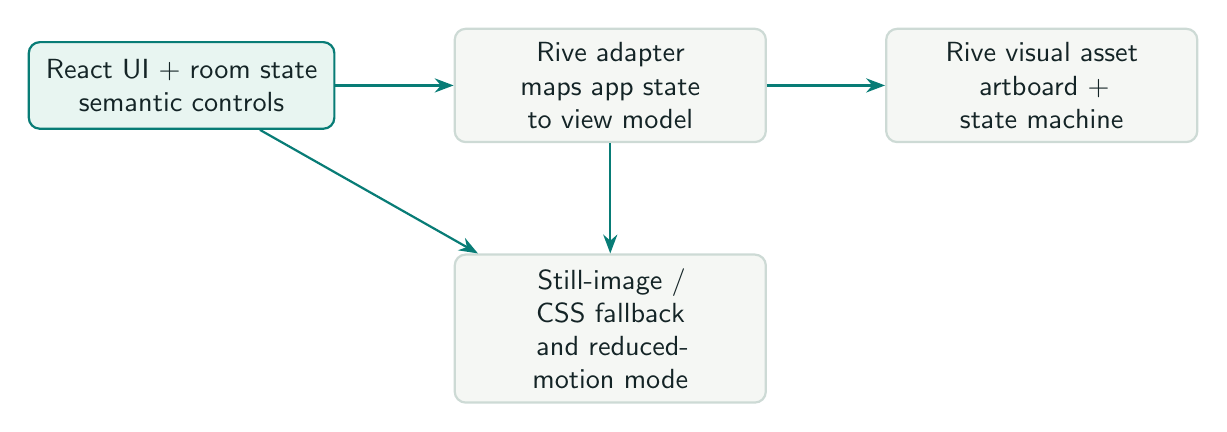
\begin{tikzpicture}[node distance=15mm]
\node[special,text width=36mm] (app) {React UI + room state\\semantic controls};
\node[phase,text width=36mm,right=of app] (adapter) {Rive adapter\\maps app state to view model};
\node[phase,text width=36mm,right=of adapter] (asset) {Rive visual asset\\artboard + state machine};
\node[phase,text width=36mm,below=14mm of adapter] (fallback) {Still-image / CSS fallback\\and reduced-motion mode};
\draw[edge] (app)--(adapter);
\draw[edge] (adapter)--(asset);
\draw[edge] (app)--(fallback);
\draw[edge] (adapter)--(fallback);
\end{tikzpicture}}
\end{center}
\textbf{Use data-binding view model properties for new assets.} Rive documents legacy state-machine inputs as deprecated for future work. Each asset still includes one artboard and a named state machine to control motion. The names below are proposed integration contracts; change them only by updating this document and implementation together.

\small
\renewcommand{\arraystretch}{1.15}
\begin{longtable}{@{}>{\raggedright\arraybackslash}p{36mm}>{\raggedright\arraybackslash}p{34mm}>{\raggedright\arraybackslash}p{60mm}>{\raggedright\arraybackslash}p{27mm}@{}}
\toprule
\textbf{Asset / placement} & \textbf{Artboard / view model} & \textbf{Properties sent by app} & \textbf{States}\\
\midrule\endfirsthead
\toprule\textbf{Asset / placement} & \textbf{Artboard / view model} & \textbf{Properties sent by app} & \textbf{States}\\\midrule\endhead
\texttt{record-indicator.riv} Solo + room recorder & \texttt{RecordIndicator} / \texttt{RecordIndicatorVM} & \texttt{phase} enum; \texttt{level} number in 0..1. Level may be 0 when no meter exists. & idle, arming, recording, saved, error\\
\texttt{pack-progress.riv} Import + conversion & \texttt{PackProgress} / \texttt{PackProgressVM} & \texttt{phase} enum; \texttt{progress} number in 0..1; \texttt{indeterminate} boolean when no total exists. & importing, converting, ready, error\\
\texttt{room-presence.riv} Lobby + recording & \texttt{RoomPresence} / \texttt{RoomPresenceVM} & \texttt{phase} enum. Visual must not imply a stranger can hear live audio. & joining, connected, reconnecting, offline\\
\texttt{showcase-cue.riv} Showcase & \texttt{ShowcaseCue} / \texttt{ShowcaseCueVM} & \texttt{phase} enum; \texttt{secondsRemaining} number, 0..5. & waiting, countdown, playing, paused, finished\\
\texttt{reaction-burst.riv} Showcase only & \texttt{ReactionBurst} / \texttt{ReactionBurstVM} & \texttt{kind} enum: clap, laugh, heart, fire; \texttt{burst} trigger. & idle, burst\\
\bottomrule
\end{longtable}
\renewcommand{\arraystretch}{1}
\normalsize
\begin{riskbox}
\textbf{Keep these out of Rive:} readable captions, creator/source credit, room code, buttons, file picker, forms, video playback, export progress text, and essential error messages. They stay in HTML for accessibility, localization, and resilience.
\end{riskbox}

\section{Rive motion and fallback rules}
\begin{itemize}
\item Document each artboard's size and maximum rendered size in Figma. Suggested slots: 24--48 px for status, 80--160 px for progress, and a bounded overlay for reactions.
\item One-shot feedback (saved, ready, burst) settles quickly; loops (recording, reconnecting) remain subtle. Motion must not obscure captions or controls.
\item Provide a still PNG/SVG and reduced-motion frame for every asset. With reduced motion, use the still frame or a quiet state change rather than a continuous loop.
\item Design an error state and a no-Rive fallback. The real text label remains beside the visual; animation never serves as the only status indicator.
\item Reaction bursts appear only when enabled by the host. The showcase works with reactions and voting disabled.
\end{itemize}

\section{Rive source, CLI, and integration acceptance}
Rive is an optional enhancement. Complete the Figma screens and components first; begin with the room countdown and recorder assets if motion work starts. For each chosen asset, deliver the editable Rive project (Editor source or RML project directory), runtime \texttt{.riv}, still fallback, and a manifest with artboard, view model, state machine, property names/types, intended slots, and timing. Do not upload or publish to a Rive workspace as part of this handoff without a separate account decision.
\begin{callout}
\textbf{Local CLI checks once assets exist}\\par
\texttt{rive <project-dir> --verify}\\par
\texttt{rive inspect <project-dir> --json}\\par
\texttt{rive <project-dir> --screenshot=preview.png}\\par
\texttt{rive <project-dir> --test}\\par
\texttt{rive <project-dir> --once} builds an unsigned \texttt{.riv} for local review. Verify intended states visually in the browser as well as through CLI output.
\end{callout}
Rive's current CLI documentation says \texttt{--publish} creates a signed asset, requires login, and may watermark output unless the file is bound to an eligible paid workspace. Keep this as a release decision, not a design dependency.

\section{Figma delivery package and acceptance}
\kicker{Deliverables}
\begin{enumerate}
\item Figma file with foundations, reusable components, desktop/phone flows, key variants, and an interactive prototype from P01 through P08. Include P09 recovery branches.
\item Exportable logo/icon artwork, original component icons, and named pack-art placeholders. Keep supplied film stills out of product branding and distributable demo assets.
\item For any chosen Rive assets: source projects, \texttt{.riv} files, still fallbacks, and a manifest matching the contract in this document.
\item Short decision notes for deliberately changed page order, mobile navigation, permission copy, room status, source attribution, or animation naming.
\end{enumerate}
\kicker{Design review checklist}
\begin{itemize}
\item A first-time player can import or join from P01 without guessing which action is primary.
\item Market cards visibly identify the original source and never imply unauthorized rehosting.
\item A long 22-line pack remains navigable on 390 px and 320 px screens.
\item Saving a take locally and submitting it to the room are visually distinct.
\item Host, performer, and spectator controls differ correctly in lobby, recording, and showcase.
\item Conversion, blocked autoplay, microphone denial, disconnect, expired room, and missing art have designed states.
\item Voting defaults off, reactions can be off, and Dub Mode has no score.
\item Every Rive visual has a static fallback and no essential text or control inside it.
\end{itemize}

\section*{References}
\addcontentsline{toc}{section}{References}
\small
Product scope: \texttt{WEBBY\_VOICER\_PLAN.md} in this project.\\
Rive CLI overview: \url{https://rive.app/docs/cli/overview}\\
Rive CLI command reference: \url{https://rive.app/docs/cli/reference/commands}\\
Rive data binding migration: \url{https://rive.app/docs/editor/data-binding/migration-guide}\\
W3C WCAG 2.2: \url{https://www.w3.org/TR/WCAG22/}\\
W3C text contrast: \url{https://www.w3.org/WAI/WCAG22/Understanding/contrast-minimum.html}\\
W3C target size: \url{https://www.w3.org/WAI/WCAG22/Understanding/target-size-minimum}
\end{document}
